\documentclass[11pt]{beamer}
\usetheme{Singapore}

\usepackage[utf8]{inputenc}
\usepackage[T1]{fontenc}
\usepackage{soul}
\usepackage{graphicx}


\graphicspath{{../Figures/}}

\def\et{{\it et al.}}


\author{Cody Glickman \\ NLM 2018}

\title{Enrichment of Bacterial Virulence Factors in Bacteriophages}

%\subtitle{}
%\logo{}

\date{ 
\includegraphics[height=2cm, width=2cm]{lablogo.png} \\ June 4th, 2018}
%\subject{}
\setbeamercovered{transparent}
\setbeamertemplate{navigation symbols}{}
\setbeamertemplate{theorems}[numbered]

\begin{document}
	\maketitle
	\begin{frame}{Outline}
	\begin{block}{Introduction}
	\end{block}
	\vspace{-0.5cm}
	\begin{block}{Baseline Virulence Factor Abundance}
	\end{block}
	\vspace{-0.5cm}
	\begin{block}{Virulence Factors in Cystic Fibrosis Phages}
	\end{block}
	\vspace{-0.5cm}
	\begin{block}{Virulence Factors in Gut with Clostridium Difficile}
	\end{block}
	\vspace{-0.5cm}
	
	\end{frame}
	%--------------------------------------------------------------------------------------

	
\section{Introduction}
\subsection{}

	\begin{frame}{Virulence}
		\begin{block}{Virulence Defined}
		The capacity of a microorganism to proliferate despite the bodies defenses
		\end{block}
		
		\begin{block}{Influences on Virulence}
		\begin{itemize}
		\item Number of microorganisms
		\item \alert{Composition of the mobile genetic reservoir}
		\item Location of niche
		\item Host immune capabilities
		\end{itemize}
		\end{block}
	
	\end{frame}
	%--------------------------------------------------------------------------------------

	\begin{frame}{Bacterial Virulence Factors Increases Pathogenesis}
	\begin{columns}
	\column{0.65\textwidth}
	\begin{block}{Examples of Virulence Factors}
		\begin{itemize}
		\item Increased fitness for nutrients
		\item Host immunity resistance
		\item Toxin secretion
		\end{itemize}
	\end{block} 
	
	\begin{block}{Pathology from Virulence Factors}
	Cholera toxin, dysentery, botulism, and food poisoning
	\end{block}
	

	\column{0.4\textwidth}
	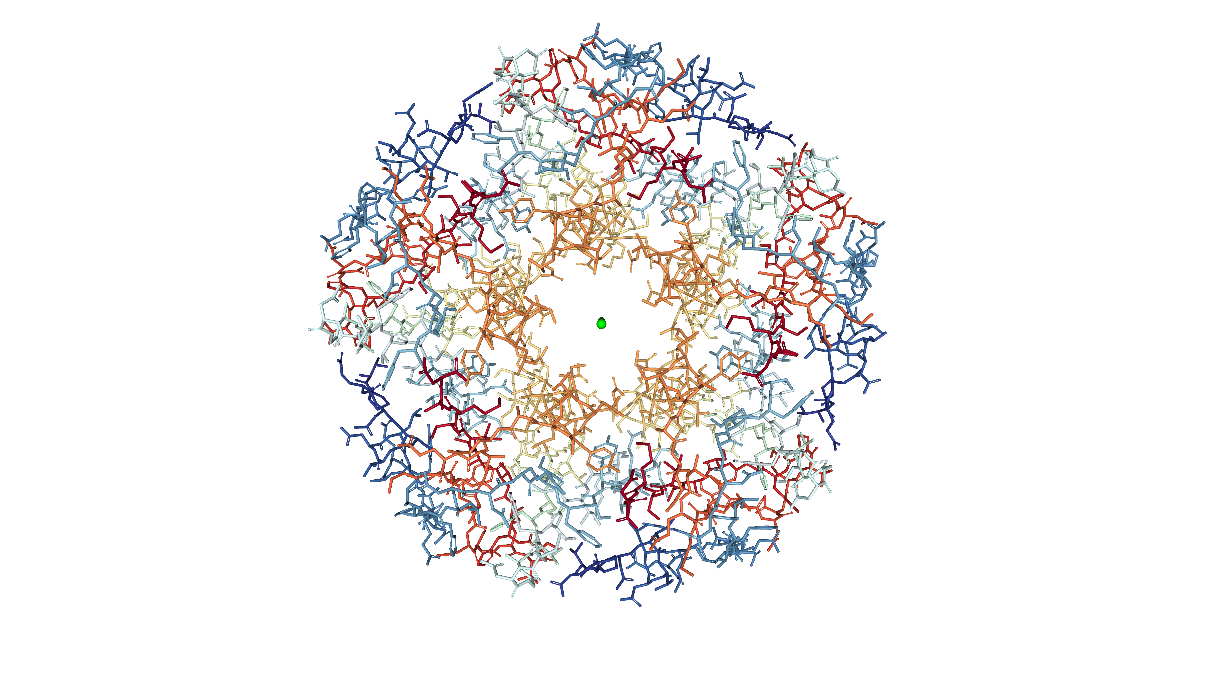
\includegraphics[height=3cm, width=5cm]{cholera.png}

	\vspace{-0.3cm}
	\hspace{0.5cm}	
	\tiny{PDB Structure of Cholera Toxin}
	\end{columns}
	
	\end{frame}
	
	%--------------------------------------------------------------------------------------
	
	\begin{frame}{Bacteriophages as a Genetic Reservoir of Virulence Factors}
	\begin{columns}
	\column{0.5\textwidth}
	\begin{block}{Bacteriophages (Phages)}
	DNA viruses that infect bacteria
	\end{block}
	
	
	\begin{block}{Bacteriophages and Pathology}
	Toxins that cause cholera, dysentery, botulism, and food poisoning all derive from bacteriophage elements.
	\end{block}
		
		
	\begin{block}{Prior Studies}
	Prior studies focus on bacteriophage relationship to disease causing bacteria
	\end{block}
	
	\column{0.5\textwidth}
	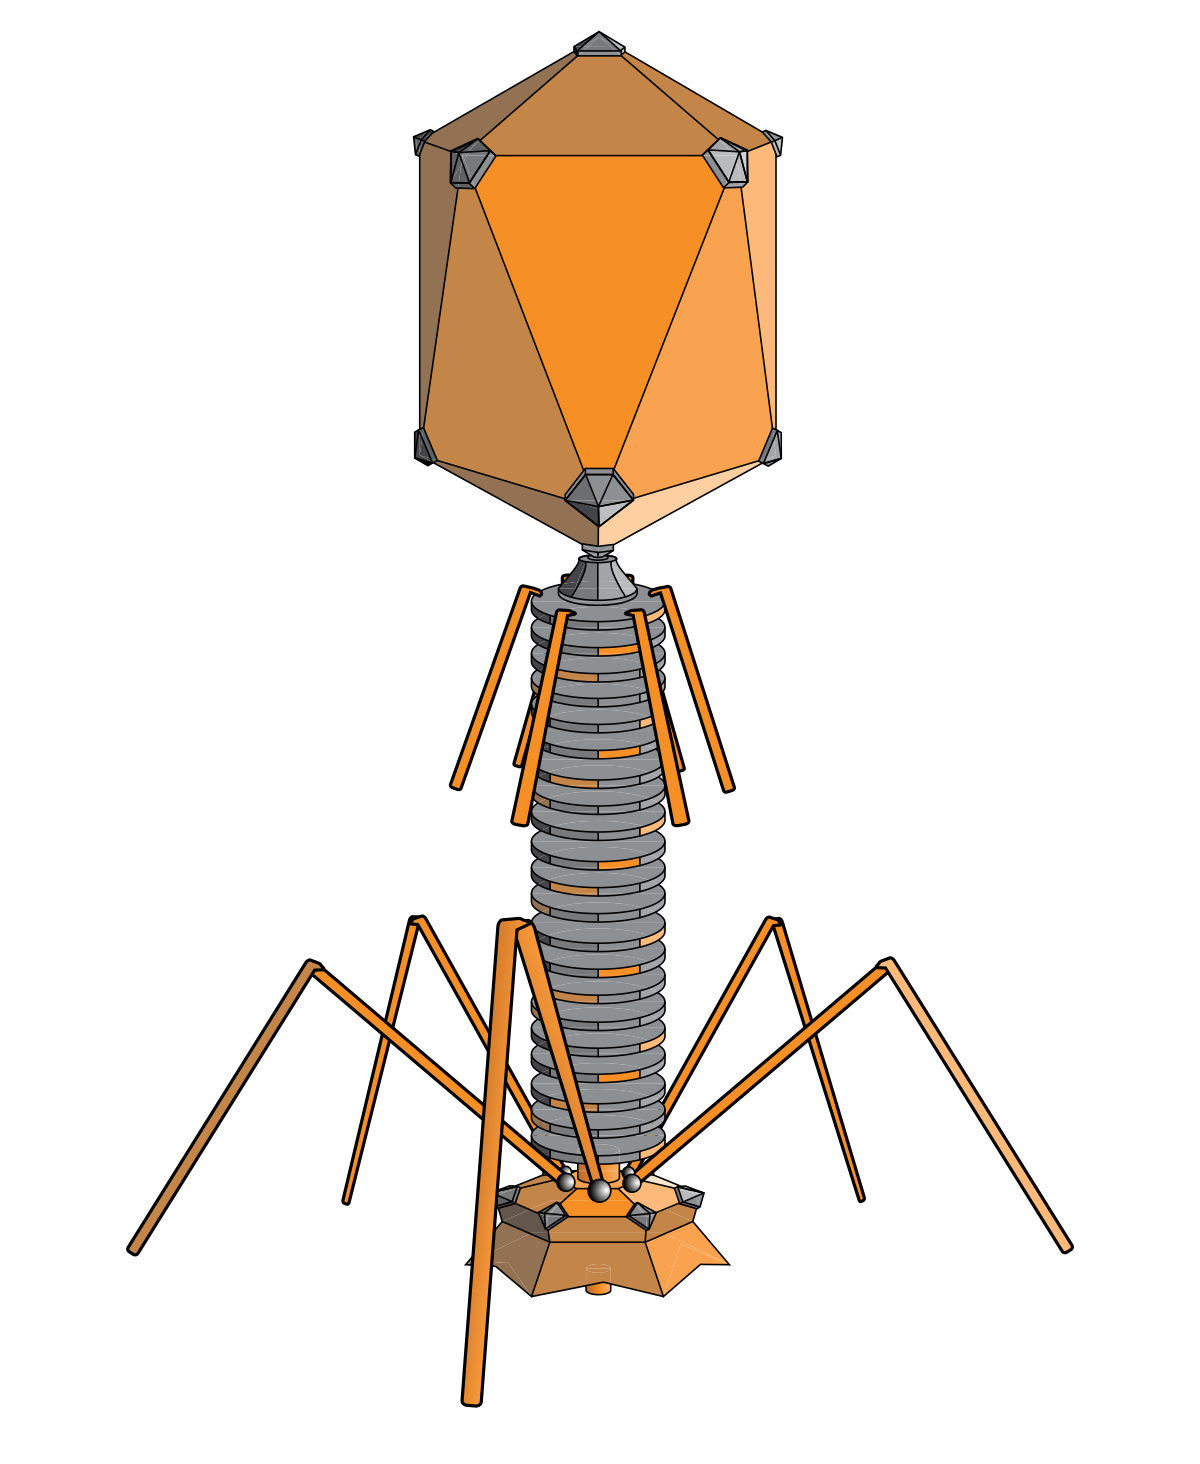
\includegraphics[height=5.5cm, width=5cm]{phage.png} \\
	\tiny{Novick, Richard, Plasmid (2003)}
	\end{columns}
		
	
	\end{frame}

	
\section{Baseline Virulence Factor Abundance}
\subsection{}

	\begin{frame}{Virulence Factor Data Acquisition}
	\begin{columns}
	\column{0.5\textwidth}
	\begin{block}{Virulence Protein Databases}
		\begin{itemize}
			\item VFDB \\ \tiny{Chen, Lihong, et al. Nucleic Acids Research (2005)}
			\item \large{PatricVF} \\ \tiny{Wattam, AR, et al. Nucleic Acids Research (2017)}
		\end{itemize}
	\end{block}
	\begin{block}{Virulence HMMs}
	\begin{itemize}
		\item pFam \\ \tiny{Bateman, Alex, et al. Nucleic Acids Research (2004)}
		\item \large{pVOG} \\ \tiny{Grazziotin, AL, et al. Nucleic Acids Research (2016)}
	\end{itemize}
		
	\end{block}
	
	
	\column{0.5\textwidth}
	\begin{block}{Phage Protein Database}
	
\includegraphics[height=3cm, width=3cm]{uniprot.png}
	\end{block}
	\end{columns}
	\end{frame}

	
	\begin{frame}{Methods}
	\begin{columns}
	\column{0.5\textwidth}
	\begin{block}{BLAST Filters}
	\begin{itemize}
	\item evalue < 10e-5
	\item pident >= 75
	\end{itemize}
	\end{block}
	
	\begin{block}{BLAST Results}
	Initial: 1484868 Hits \\
	Post-filtering: 5022 Hits
	\end{block}
	
	\column{0.5\textwidth}
	\begin{block}{HMM Filters}
	\begin{itemize}
	\item MSV filter
	\item bias filter
	\item Vit filter 
	\item Fwd filter
	\end{itemize}
	\end{block}
	
	\begin{block}{HMM Results}
	Post-filtering: 15389 Hits
	\end{block}

	\end{columns}
	\end{frame}
	
	\begin{frame}{Hit Count Distribution}
	\begin{columns}
	\column{0.5\textwidth}
	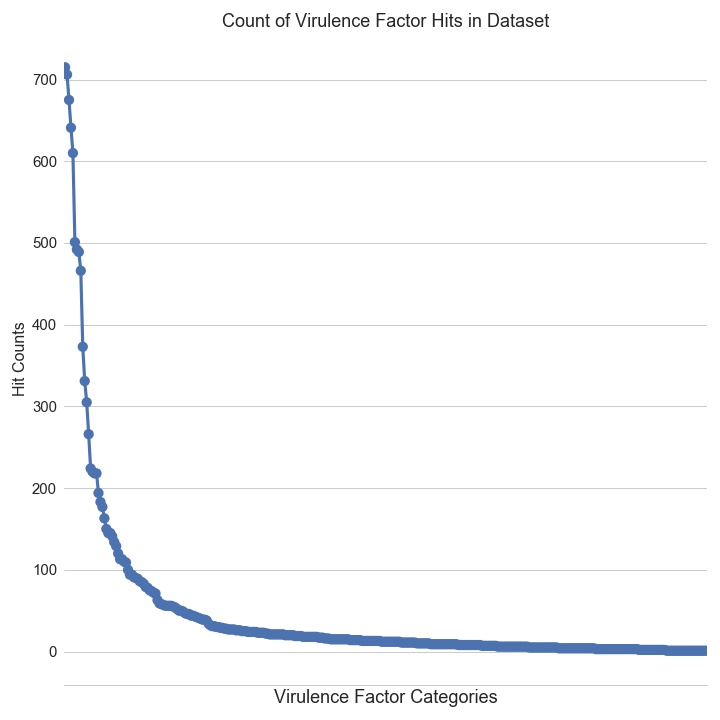
\includegraphics[height=5cm, width=5cm]{HMM_Hit_Counts.jpg}
	\column{0.5\textwidth}
	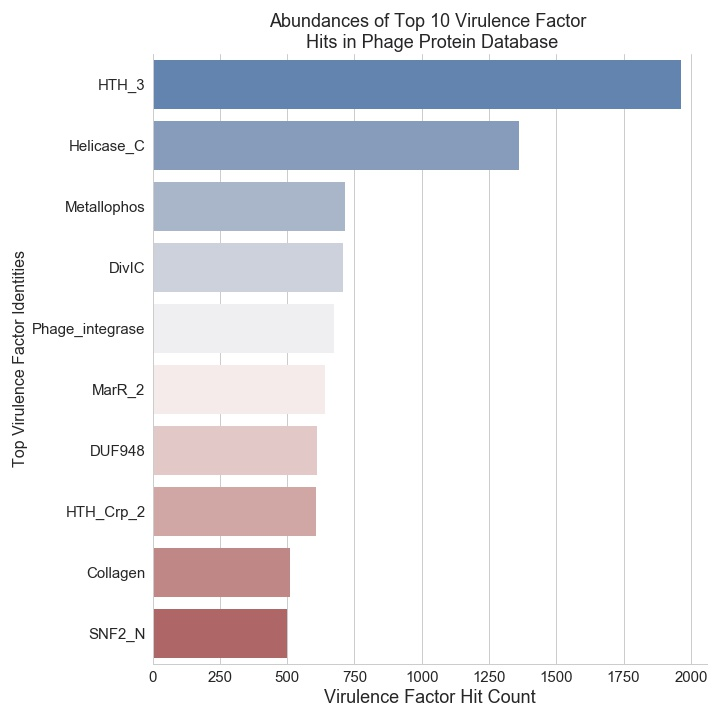
\includegraphics[height=6cm, width=6cm]{Top_VF_Hit_Plot.jpg}
	\end{columns}
	\end{frame}
	
	
	\begin{frame}{All Phages Distribution of VF Gene Percentages}
	\begin{columns}
	\column{0.5\textwidth}
	\large{BLAST}
	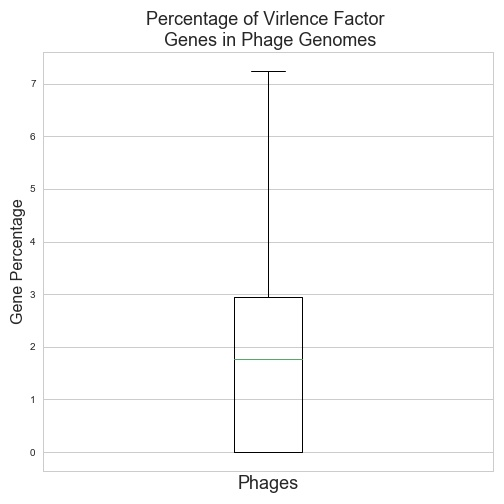
\includegraphics[height=5cm, width=5cm]{All_Phages_BLAST_Percentage.jpg}
	\column{0.5\textwidth}
	\large{HMM}
	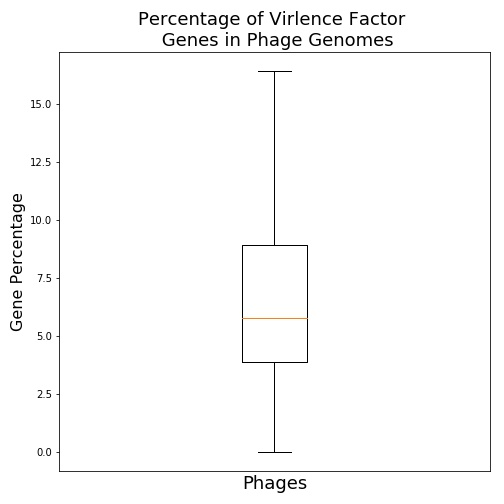
\includegraphics[height=5cm, width=5cm]{All_Phages_Percentage.jpg}
	\end{columns}
	\end{frame}
	
	\begin{frame}{Top Phage Distributions}
	\begin{columns}
	\column{0.5\textwidth}
	\large{BLAST}
	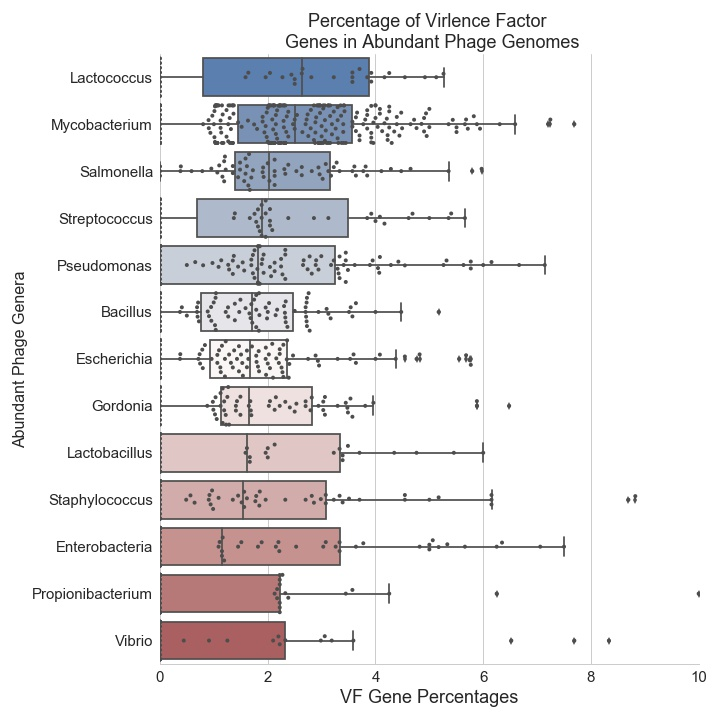
\includegraphics[height=5cm, width=5cm]{Top_Phages_Percentage_BLAST.jpg}
	\column{0.5\textwidth}
	\large{HMM}
	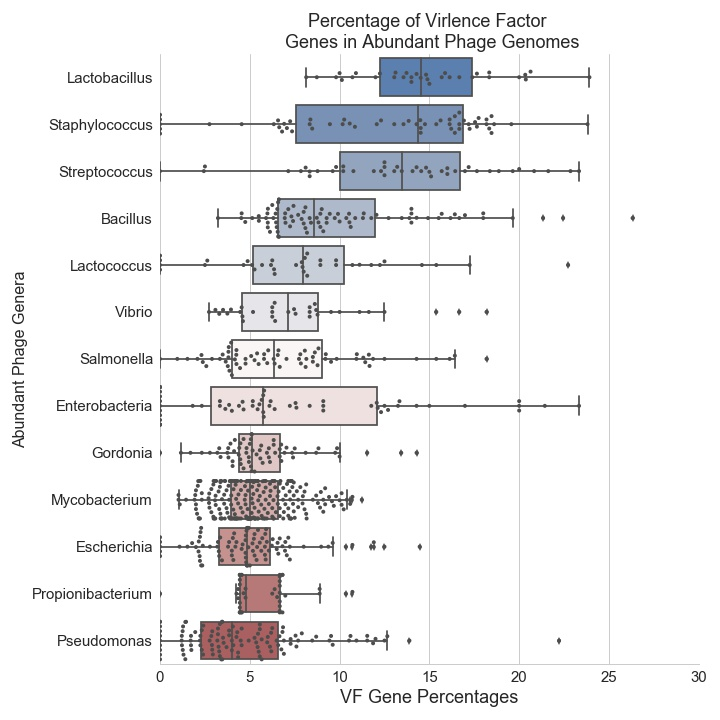
\includegraphics[height=5cm, width=5cm]{Top_Phages_Percentage_HMM.jpg}
	\end{columns}
	\end{frame}
	
	

\section{Virulence Factors in Cystic Fibrosis Phages}
\subsection{}

	
	\begin{frame}{Clinical Data and Methodology}
	\begin{block}{Data Source}
	The data consists of 5 normal and 5 CF viromes
	\end{block}
	\end{frame}

	
	
	
\section{}

	\begin{frame}{Concluding Remarks}
	\begin{columns}
	\column{0.3\textwidth}
	\begin{block}{Base line}
	Established Baseline
	\end{block}
	\column{0.3\textwidth}
	\begin{block}{GRAB}
	Viral GRAB will contribute to a focus on phages specific to lung infections
	\end{block}
	
	\end{columns}
	
	\end{frame}
	
	
	
	
	\begin{frame}{}
	\vspace{1cm}
	{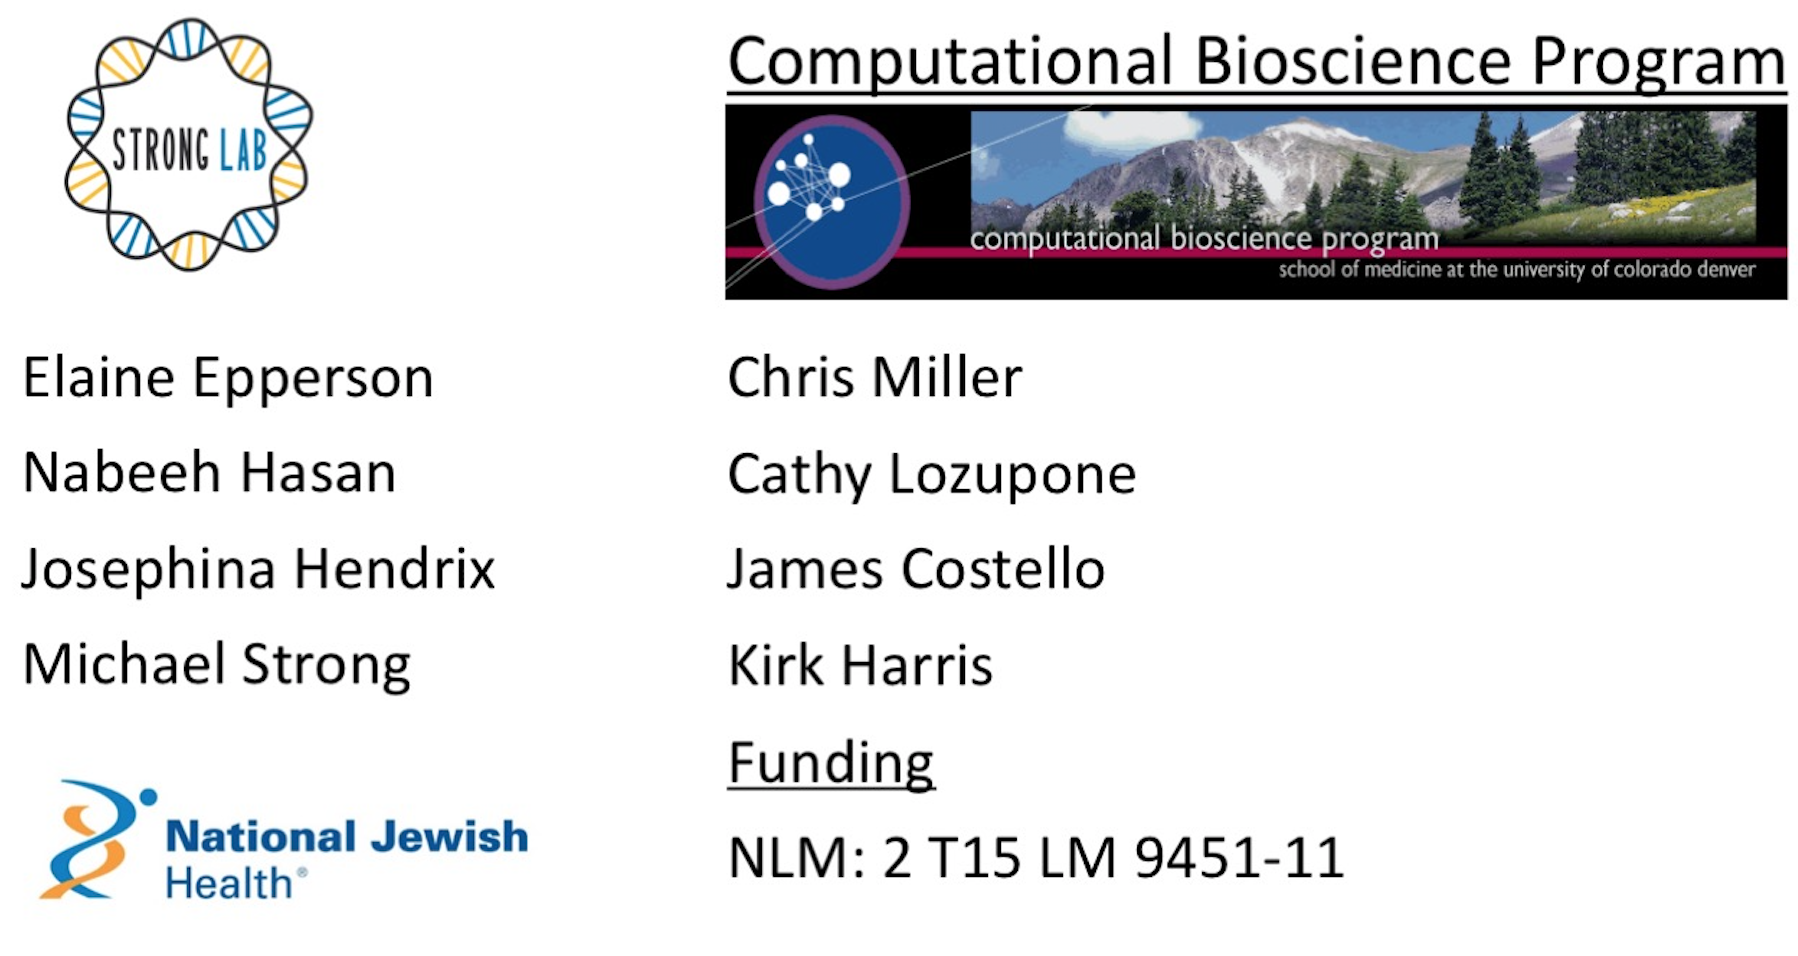
\includegraphics[height=8cm, width=11cm]{Acknowledgements.png} }
	\end{frame}
	
	
	\begin{frame}{Questions?}
	\center
	Cody Glickman \\ 
\includegraphics[height=2cm, width=2cm]{lablogo.png} \\ cody.glickman@ucdenver.edu \\ \alert{www.github.com/glickmac} \\ www.codyglickman.com
	\end{frame}
	



\end{document}